\documentclass[tikz]{standalone}
\begin{document}
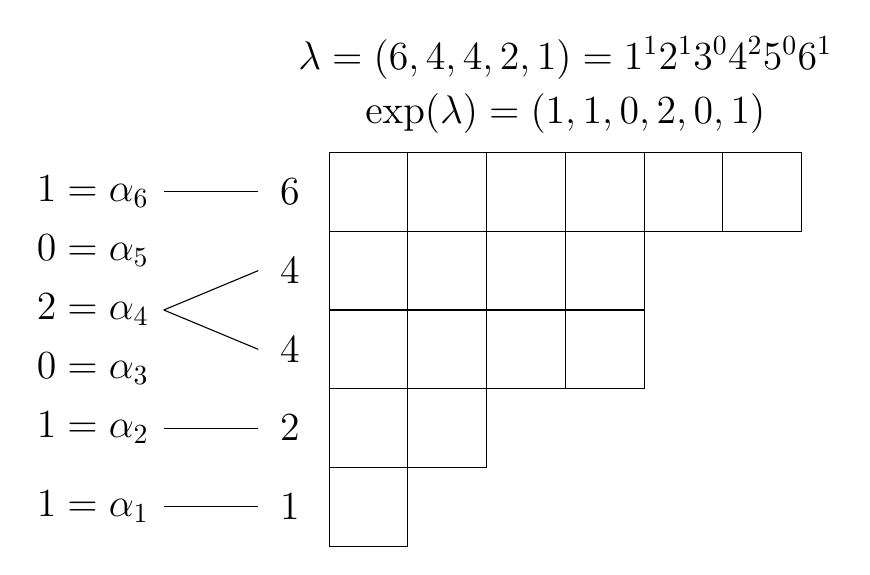
\begin{tikzpicture}
\begin{scope}[local bounding box=scope1]
  \draw (0,0) -- (6,0);\draw (0,-1) -- (6,-1);\draw (0,-2) -- (4,-2);\draw (0,-3) -- (4,-3);\draw (0,-4) -- (2,-4);\draw (0,-5) -- (1,-5);\draw (1,0) -- (1,-5);\draw (2,0) -- (2,-4);\draw (3,0) -- (3,-3);\draw (4,0) -- (4,-3);\draw (5,0) -- (5,-1);\draw (6,0) -- (6,-1);\draw (0,0) -- (0,-5);
\end{scope}
\begin{scope}[font=\Large, shift={(-0.5,-0.5)}]
  \draw (0,0) node{6};\draw (0,-1) node{4};\draw (0,-2) node{4};\draw (0,-3) node{2};\draw (0,-4) node{1};
  \draw (-2.5,0) node{$1=\alpha_{6}$};\draw (-2.5,-0.75) node{$0=\alpha_{5}$};\draw (-2.5,-1.5) node{$2=\alpha_{4}$};\draw (-2.5,-2.25) node{$0=\alpha_{3}$};\draw (-2.5,-3) node{$1=\alpha_{2}$};\draw (-2.5,-4) node{$1=\alpha_{1}$};
  \draw (-0.4,0) -- (-1.6,0);\draw (-0.4,-1) -- (-1.6,-1.5);\draw (-0.4,-2) -- (-1.6,-1.5);\draw (-0.4,-3) -- (-1.6,-3);\draw (-0.4,-4) -- (-1.6,-4);
\end{scope}
\begin{scope}[font=\Large, shift={(scope1.north)}]
  \draw (0,1.2) node{$\lambda = (6,4,4,2,1)=1^{1}2^{1}3^{0}4^{2}5^{0}6^{1}$};
  \draw (0,0.5) node{$\exp(\lambda)=(1,1,0,2,0,1)$};
\end{scope}
\end{tikzpicture}
\end{document}
